\newcommand{\booktitle}{User Manual}
\newcommand{\tocname}{Contents}
\newcommand{\figword}{Figure}
\newcommand{\chapterword}{Chapter \thesection}
\newcommand{\coverline}{Reading and plotting one-dimensional output}
\newcommand{\covercaption}{Cell-centre position in micrometres. The three curves follow the same synthetic temperature peak at successive recorded times.}
\newcommand{\editionline}{Desktop edition \enspace 2.3.1}
\newcommand{\manualdate}{November 2026}
\newcommand{\creditline}{English edition \enspace ·\enspace Software by Bo Xu}
% Compile either edition from its own directory with XeLaTeX.
\documentclass[11pt,a4paper]{article}
\usepackage[top=22mm,bottom=23mm,left=22mm,right=22mm,headheight=16pt,footskip=12mm]{geometry}
\usepackage{fontspec,xeCJK}
\setmainfont{TeX Gyre Pagella}
\setsansfont{TeX Gyre Heros}
\setmonofont[Scale=0.88]{Latin Modern Mono}
\IfFileExists{C:/Windows/Fonts/msyh.ttc}
  {\setCJKmainfont[AutoFakeBold=2]{SimSun}\setCJKsansfont{Microsoft YaHei}\setCJKmonofont{Microsoft YaHei}}
  {\setCJKmainfont[BoldFont=FandolSong-Bold.otf]{FandolSong-Regular.otf}%
   \setCJKsansfont[BoldFont=FandolHei-Bold.otf]{FandolHei-Regular.otf}\setCJKmonofont{FandolHei-Regular.otf}}
\usepackage{graphicx,xcolor,booktabs,tabularx,array,enumitem,fancyhdr,tikz}
\usepackage{hyperref}
\definecolor{ink}{HTML}{182F40}
\definecolor{teal}{HTML}{006D72}
\definecolor{muted}{HTML}{425B66}
\definecolor{rulecol}{HTML}{B6D0CF}
\definecolor{wash}{HTML}{EEF5F4}
\hypersetup{unicode=true,colorlinks=true,linkcolor=teal,urlcolor=teal,bookmarksnumbered=true,bookmarksdepth=2,
 pdfauthor={MULTI1Dvisual},pdftitle={MULTI1Dvisual 2.3.1 — \booktitle}}
\urlstyle{same}
\setlength{\parindent}{0pt}
\setlength{\parskip}{5.5pt}
\linespread{1.10}
\setlist[enumerate]{leftmargin=1.9em,label=\textcolor{teal}{\sffamily\bfseries\arabic*.},itemsep=3pt,topsep=4pt,parsep=0pt}
\setcounter{tocdepth}{1}
\renewcommand{\contentsname}{\tocname}
\pagestyle{fancy}\fancyhf{}
\fancyhead[L]{\small\sffamily\bfseries\color{teal}MULTI1Dvisual}
\fancyhead[R]{\small\sffamily\color{muted}\nouppercase{\leftmark}}
\fancyfoot[L]{\footnotesize\sffamily\color{muted}\booktitle\enspace ·\enspace 2.3.1}
\fancyfoot[R]{\sffamily\bfseries\color{teal}\thepage}
\renewcommand{\headrulewidth}{0.4pt}
\renewcommand{\headrule}{{\color{rulecol}\hrule height \headrulewidth width\headwidth}}
\raggedbottom
\setlength{\emergencystretch}{2em}
\newcommand{\chapterpage}[2]{\clearpage\refstepcounter{section}\label{#1}%
 \addcontentsline{toc}{section}{\protect\numberline{\thesection}#2}\markboth{#2}{}%
 {\sffamily\bfseries\color{teal}\chapterword\par}\vspace{0.5mm}
 {\sffamily\bfseries\color{ink}\fontsize{24}{30}\selectfont #2\par}\vspace{2mm}}
\newcommand{\nextpage}[2]{\clearpage\phantomsection\label{#1}%
 \pdfbookmark[2]{#2}{sub:#1}%
 {\sffamily\bfseries\color{teal}\chapterword\par}\vspace{0.5mm}
 {\sffamily\bfseries\color{ink}\fontsize{22}{28}\selectfont #2\par}\vspace{2mm}}
\newcommand{\subhead}[1]{\par\addvspace{2.5mm}{\large\sffamily\bfseries\color{teal}#1\par}\nobreak}
\newcommand{\ui}[1]{{\sffamily\bfseries\color{ink}#1}}
\newcommand{\code}[1]{{\ttfamily\detokenize{#1}}}
\newcommand{\keys}[1]{{\small\sffamily\bfseries #1}}
\newcommand{\checknote}[2]{\par\addvspace{2.5mm}\noindent\colorbox{wash}{%
 \parbox{\dimexpr\linewidth-2\fboxsep\relax}{\vspace{1mm}\hspace{1.4mm}%
 \begin{minipage}{\dimexpr\linewidth-3mm\relax}{\sffamily\bfseries\color{teal}#1}\enspace #2\end{minipage}\vspace{1.4mm}}}\par}
\newcommand{\Table}[3]{\par\smallskip\begingroup\small\renewcommand{\arraystretch}{1.24}%
 \begin{tabularx}{\linewidth}{@{}>{\raggedright\arraybackslash}p{.295\linewidth}>{\raggedright\arraybackslash}X@{}}\toprule
 \sffamily\bfseries\color{teal}#1 & \sffamily\bfseries\color{teal}#2\\\midrule #3\bottomrule
 \end{tabularx}\endgroup\par}
\newcounter{manualfig}
\newcommand{\Figure}[3]{\par\addvspace{2mm}\stepcounter{manualfig}\begingroup\centering
 \includegraphics[width=\linewidth,height=#3,keepaspectratio]{images/#1.png}\par
 \endgroup{\small\color{muted}{\sffamily\bfseries\color{teal}\figword\ \themanualfig.}\enspace #2\par}\smallskip}
\newcommand{\repo}{\href{https://github.com/boxu-pku/MULTI1Dvisual}{GitHub · boxu-pku/MULTI1Dvisual}}
\newcommand{\cover}{\thispagestyle{empty}\vspace*{6mm}
 
\includegraphics[width=27mm]{../../resources/icons/multi1dvisual.png}\par\vspace{9mm}
 {\sffamily\bfseries\color{ink}\fontsize{38}{44}\selectfont MULTI1Dvisual\par}
 {\sffamily\bfseries\color{teal}\fontsize{28}{37}\selectfont\booktitle\par}
 \vspace{3mm}{\Large\color{muted}\coverline\par}
 \vfill
 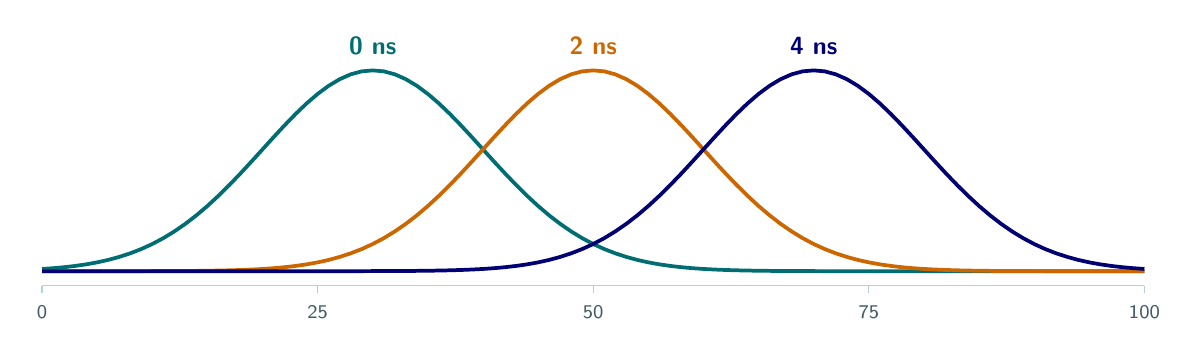
\begin{tikzpicture}[x=.140cm,y=.51cm]
 \draw[rulecol] (0,0)--(100,0);
 \foreach \p in {0,25,50,75,100} {
  \draw[rulecol] (\p,0)--(\p,-.18);
  \node[below,font=\scriptsize\sffamily,text=muted] at (\p,-.25){\p};}
 \foreach \p/\col/\name in {30/teal/0,50/orange!80!black/2,70/blue!45!black/4}{
  \draw[line width=1.35pt,color=\col] plot[domain=0:100,samples=101] (\x,{.36+5*exp(-((\x-\p)^2)/200)});
  \node[above,font=\small\sffamily\bfseries,text=\col] at (\p,5.52){\name\ ns};}
 \end{tikzpicture}\par
 {\small\color{muted}\covercaption\par}
 \vfill{\color{rulecol}\rule{\linewidth}{0.8pt}}\par
 {\large\sffamily\bfseries\color{ink}\editionline}\hfill{\sffamily\color{muted}\manualdate}\par
 {\small\color{muted}\creditline}\clearpage}
\newcommand{\contentspage}{\markboth{\tocname}{}\pdfbookmark[1]{\tocname}{contents}%
 \tableofcontents}

\begin{document}\color{ink}
\cover
\contentspage
\subhead{Using this manual}
If this is your first session, install the desktop application and work through the example in Chapter~\ref{quick}. Keep the example open as you read the three plotting chapters. Chapter~\ref{export} explains how to identify the values in each exported table.
\checknote{Files to keep together}{Both editions use the same \code{quickstart.zip}. The archive is linked at the top of the project README and included with the desktop installers. The screenshots show the English Qt interface on Windows. Linux uses the same plotting controls. Some dialogs retain Chinese labels in the English interface.}
\chapterpage{install}{Install the desktop application}
\subhead{Linux packages}
Use the package built for your distribution. These installers register an application menu entry and use the distribution's Python, Qt and plotting libraries. Allow the package manager to fetch the dependencies it lists.
\Table{Distribution}{File for version 2.3.1}{
Debian or Ubuntu & \code{multi1dvisual_2.3.1-1_all.deb}\\
Fedora & \code{multi1dvisual-2.3.1-1.noarch.rpm}\\}
\begin{enumerate}
\item Open the downloaded file in your file manager. If it displays the archive contents, use \ui{Open With} and choose the system's software installer, such as GDebi on Ubuntu when installed.
\item Review the package name \code{multi1dvisual} and choose \ui{Install}. System-wide installation can prompt for your administrator password.
\item Find \ui{MULTI1Dvisual} in the applications menu, or run \code{multi1dvisual} in a terminal within your graphical session.
\item The main window opens with three plotting tabs. From \ui{Help → Documentation}, choose either manual to open it locally in a PDF reader.
\end{enumerate}
\subhead{Terminal installation}
Open a terminal in the directory containing the downloaded package. Use the command for your distribution. The \code{./} selects the local file.
\begin{verbatim}
sudo apt install ./multi1dvisual_2.3.1-1_all.deb
\end{verbatim}
\begin{verbatim}
sudo dnf install ./multi1dvisual-2.3.1-1.noarch.rpm
\end{verbatim}
\subhead{Check, update or remove}
On Debian or Ubuntu, \code{dpkg-query -W multi1dvisual} prints the installed version. On Fedora, use \code{rpm -q multi1dvisual}. For a newer package, repeat the installation command with its new filename. To uninstall, use \code{sudo apt remove multi1dvisual} or \code{sudo dnf remove multi1dvisual}.
\checknote{Offline documentation}{Find the manuals under \code{/usr/share/multi1dvisual/docs/}. Copy \code{examples/quickstart.zip} from there to a writable directory for the exercises.}

\nextpage{otherinstall}{Windows and source installations}
\subhead{Windows 10 or 11, x64}
\begin{enumerate}
\item Open \code{MULTI1Dvisual-Setup-2.3.1-x64.exe}. Select the installer language and the optional desktop shortcut.
\item Finish the wizard and launch \ui{MULTI1Dvisual} from Start. This installer includes Python and the plotting libraries.
\item Use \ui{Help → Documentation} for the PDFs. In the default installation, enter \texttt{\%LOCALAPPDATA\%} in the File Explorer address bar, then open \code{Programs/MULTI1Dvisual/manual/docs}. The \code{examples} folder contains the practice archive.
\end{enumerate}
Use \ui{Installed apps} in Windows Settings to uninstall. If you chose a custom installation directory, look for \code{manual/docs} under that directory.
\subhead{Run a source checkout on Linux}
For a checkout that contains \code{main.py} and \code{requirements.txt}, run the following from the project root in a graphical session. The Python installation must provide the \code{venv} module.
\begin{verbatim}
python3 -m venv .venv
. .venv/bin/activate
python -m pip install -r requirements.txt
python main.py
\end{verbatim}
The source checkout keeps the PDFs under \code{docs/manual_EN} and \code{docs/manual_CN}, and the example in \code{docs/examples}. For building native packages from a checkout, see \code{packaging/README.md} in that checkout.
\subhead{Set the interface language}
Choose \ui{Help → Change Language} (帮助 → 更改语言 in the Chinese interface). Select \ui{English} or \ui{简体中文}, confirm and restart the application. Saving an installer language and choosing an application language are separate steps.
\checknote{First launch}{A blank canvas is expected. Use \keys{Ctrl+O} to load a data file, then choose a variable and press \ui{Plot}. The complete example starts on the next page.}

\chapterpage{quick}{Quick start with the sample data}
Extract \code{quickstart.zip} into a writable folder. The bundle contains two representations of a small, synthetic temperature distribution on a stationary grid. You can check every plotted maximum against the numbers below.
\begin{enumerate}
\item Press \keys{Ctrl+O} and open \code{quickstart.case}. Keep the two matching \code{.dat} files beside it. Check the file information bar for \ui{9} timesteps and \ui{21} cells.
\item Press \keys{Ctrl+1}. Choose \ui{T}, coordinate \ui{XC}, position unit \ui{um} and value unit \ui{eV}. Hold Ctrl and select moments \ui{\#0}, \ui{\#4} and \ui{\#8}. Click \ui{Plot}. The three peaks move to the right.
\item Press \keys{Ctrl+2}. Choose the cell time-evolution mode, \ui{T} and \ui{Cell \#10}. Use \ui{ns} and \ui{eV}, then click \ui{Plot}. Its largest sampled value occurs at 2~ns.
\item Press \keys{Ctrl+3}. Choose \ui{T}, \ui{XC} and time on the horizontal axis. Select \ui{viridis}, click \ui{Auto} in the colour settings, then \ui{Plot}. Trace the bright band from 30 to 70~µm.
\item Return to the spatial tab, retain the three moments and use \ui{Export Data} to save \code{profiles.csv}. Open the table and compare the values below. To keep a picture as well, use \keys{Ctrl+S} and give the file a \code{.png} extension.
\end{enumerate}
\Table{Selected moment}{Expected maximum of T on the sampled grid}{
\#0 \enspace 0.0 ns & 8 eV at 30 µm, cell \#6\\
\#4 \enspace 2.0 ns & 8 eV at 50 µm, cell \#10\\
\#8 \enspace 4.0 ns & 8 eV at 70 µm, cell \#14\\}
\subhead{What the example contains}
There are nine outputs at 0.5~ns intervals. The 21 centres run from 0 to 100~µm at 5~µm intervals. \code{T} is a smooth peak above a 2~eV baseline. \code{R} is a simple density ramp. The global scalar \code{ENIE} increases from 10 to 18 in the example's stored units.
\checknote{Other practice inputs}{\code{quickstart.out} holds the same temperature data in binary form for Chapter~\ref{recorder}. A separate folder, \code{moving-edge/}, contains the density example for Chapters~\ref{shock} and~\ref{standard}.}

\chapterpage{files}{Open files and navigate the workspace}
\Table{Entry to open}{Companion data and how the viewer reads it}{
\code{fort.10} or binary \code{.out} & Open the output file directly. Its records contain the stored coordinates, fields and time samples.\\
Formatted \code{fort.10} & The viewer checks the initial record to distinguish supported MULTI-IFE formatted text from standard binary output. Preserve the producer's original filename.\\
\code{name.case} & The basename locates \code{name.scalars.dat} and \code{name.center.dat} in the same directory. Both are required.\\
Additional ASCII tables & \code{name.interface.dat} supplies interface fields, while \code{name.group.dat} can supply group data when present.\\}
\subhead{Check the ASCII layout}
The example tables are tab-separated. A header beginning with \texttt{\# TIME} names the columns. The scalar table has one row per output time. Centre rows are grouped in the same time order, with the same number of cells in every block. The reader reshapes these rows by count. Changing their order in a spreadsheet can associate a value with the wrong cell.
\subhead{Read the main window}
The top information bar shows the active filename and the timestep and cell counts. The left side of each tab holds its controls and the right side holds the plot. Scroll the controls if the plotting and export buttons are below the visible area. The bottom status line reports loads, plots and saves.
\begin{enumerate}
\item \keys{Ctrl+O} opens the file picker. The English button reads \ui{Open Binary File...}. The supported-file filter includes \code{.case}.
\item To refresh data written since opening the file, choose \ui{Reload} in the top bar or toolbar. After loading, reselect the variable and records, then plot again.
\item Opening another file changes the active dataset. Check the filename before exporting or starting a recording.
\end{enumerate}
\checknote{One export direction}{The legacy ASCII export creates \code{_SCout.txt} and \code{_TSout.txt}. To open a decimal case, use the original \code{.case} and its matching \code{.dat} files.}

\nextpage{coords}{Choose coordinates and units}
First decide what is held fixed. The spatial tab fixes an output time. A cell history fixes an array index. A fixed-position cut through a moving grid can pass through different cells over time.
\Table{Coordinate}{Meaning and appropriate use}{
\code{XC} / \code{X} & Current cell centre / interface position. Use a length unit. The grid can move between outputs. Match a field to its stored location.\\
\code{LC} / \code{LI} & Centre / interface position at the first output. This initial length coordinate gives each indexed location a fixed reference.\\
\code{NC} / \code{NI} & Cell / interface number from the file. The axis shows stored index labels. They can differ from the zero-based \ui{Cell \#} picker.\\
\code{CMC} / \code{CMI} & Cumulative mass coordinate at centres / interfaces, when available. The axis unit is mass per area.\\}
The selector lists the coordinates supplied or derivable for the file. A centre field commonly has \(N\) values and an interface field \(N+1\). Compare a centre temperature with \code{XC}. For an interface field stored on \code{X}, select \code{X} and check its array length before interpreting an endpoint.
\subhead{Units on the controls}
\code{um} denotes micrometres. \(1~\mathrm{cm}=10^4~\mathrm{\mu m}\) and \(1~\mathrm{ns}=10^{-9}~\mathrm{s}\). The temperature control for \code{T}, \code{TI} and \code{TR} offers eV and K. The application uses 11,604.518~K per eV. The example peak is therefore about 92,836~K. Pressure controls for \code{P} and \code{PT} include GPa, Mbar and the stored \code{dyn/cm^2}. Read the time, coordinate and value units independently.
\subhead{Match the index to the question}
In the example, \ui{Cell \#10} is the eleventh centre, at 50~µm. The \code{NC} value there is 11. The time-history picker keeps following index 10 if that centre moves. To sample a constant spatial position instead, use a fixed-position profile in Chapter~\ref{profiles}.
\checknote{Unit changes}{Replot after changing a unit. On a heatmap, also recalculate or re-enter the colour limits in the chosen value unit before comparing two figures.}

\chapterpage{spatial}{Compare spatial profiles}
Use \ui{Spatial Plot} (\keys{Ctrl+1}) to compare one field at several recorded times. Each list entry shows a zero-based record number and its time in ns.
\begin{enumerate}
\item With \code{quickstart.case} open, choose \ui{T}, \ui{XC}, \ui{um} and \ui{eV}. Select moment \ui{\#0}, choose blue and a solid line, then apply the style to the selection.
\item Give \ui{\#4} an orange dashed line and \ui{\#8} a purple dash-dot line in the same way. Ctrl-click the three moments, enable \ui{Show Legend} and click \ui{Plot}.
\end{enumerate}
\Figure{spatial}{The same field at 0, 2 and 4 ns. The legend identifies the times. The three sampled maxima have the same height and different positions.}{110mm}
Use \ui{Select All} or inverse selection for long lists. Removing a selected moment marks it as excluded. Restore it with \ui{Cancel Delete} or the corresponding restore control, then select and replot. These controls work on the selection in memory. The loaded data file is preserved.
\checknote{Read a moving grid}{The plot uses each record's own \code{XC} or \code{X} when available. A spatial CSV uses one coordinate column for all selected times. The export example on page~\pageref{checkcsv} explains how to handle this difference.}

\chapterpage{temporal}{Read a time history}
Open \ui{Temporal Plot} (\keys{Ctrl+2}). A global variable gives one stored value per output. In cell mode, each selected cell contributes a separate series from a spatial field.
\begin{enumerate}
\item In global mode, choose \ui{ENIE}, set time to \ui{ns} and click \ui{Plot}. The example gives 10, 14 and 18 at 0, 2 and 4 ns.
\item Switch to cell time evolution, choose \ui{T}, value unit \ui{eV} and \ui{Cell \#10}. Enable the legend and click \ui{Plot}. For a comparison, add cells \ui{\#6} and \ui{\#14} with Ctrl-click and replot.
\end{enumerate}
\Figure{temporal}{Cell \#10 sampled at all nine times. On this stationary grid, this cell is also the fixed position 50 µm.}{110mm}
Use distinct colours or line styles and apply them to selected cells before plotting. The material-colour action uses stored material IDs (\code{MID}) where available. The practice bundle has no material IDs. The global series takes its style from the controls for the current plot.
\checknote{Compare with a table}{Use this tab's \ui{Export Data} to get one time column and one column per enabled selected cell. At 2 ns, \ui{Cell \#10} has 8 eV. The global export instead names its second column after the scalar.}

\chapterpage{heatmap}{Build a space–time heatmap}
A heatmap assigns a colour to a field value at a time and coordinate. Start with the same field and units as your line plots so the colour bar has a direct numerical reference.
\begin{enumerate}
\item Open \ui{Heatmap} (\keys{Ctrl+3}). Select \ui{T}, \ui{XC}, \ui{um}, \ui{ns} and \ui{eV}. Under coordinate direction, put time on X and position on Y.
\item Choose \ui{viridis}. Click \ui{Auto} in the colour settings to fill the minimum and maximum, leave linear colour enabled and click \ui{Plot}.
\end{enumerate}
\Figure{heatmap}{Time runs left to right. The bright ridge passes through approximately 50 µm at 2 ns. The scale at the right gives temperature in eV.}{110mm}
To mark a reading, enter \code{50} under \ui{Position Marks} and \code{2} under \ui{Time Marks}, then plot again. Enter multiple values with commas. The physical meanings of the mark fields stay the same when the axes are exchanged.
\checknote{Read an axis before clicking}{In this orientation the point at 2 ns and 50 µm has screen coordinates \((2,50)\). When position is on X and time is on Y the same point is \((50,2)\).}

\nextpage{sampling}{Colour limits, zoom and sampling}
\subhead{Compare two maps on a common scale}
\begin{enumerate}
\item Plot the example with \ui{T} in eV. Use \ui{Auto} once to learn the range. Enter 2 and 8 as the colour minimum and maximum and plot again.
\item Open the comparison data and reselect the same field, coordinate, units, colour map and limits. Apply the same axis ranges when comparing positions or durations across files.
\item For positive quantities spanning a large range, enable \ui{Log Color} and choose a strictly positive minimum below the maximum. Keep a linear colour scale to inspect zero crossings or signed values.
\end{enumerate}
The X and Y range controls limit the visible plot. Colour limits govern the mapping of values to colours. Values above a fixed maximum can share the same colour. Inspect a line plot or CSV if you need to distinguish their numerical values.
\subhead{What lies between recorded points}
For physical-position maps, the viewer linearly interpolates each record's field onto a common spatial grid, using the coordinates at that record. Areas outside the sampled support can be blank. In time-horizontal mode it can also interpolate along time. The display grid can be much denser than the original array of 9 times by 21 centres.
For a stored mass or number coordinate (\code{CMC}, \code{CMI}, \code{NC}, \code{NI}), the labelled cells or interfaces share fixed coordinates between records. An optional \ui{I-Left} or \ui{I-Right} multi-group spectrum uses time and group frequency instead of spatial position, when frequency-group centres and matching data are present.
\subhead{Navigate the plotting canvas}
Drag a rectangle with the left mouse button to frame a region. The scroll wheel changes the range around the pointer. Click the canvas and press \keys{H} to step back through zoom history or \keys{A} for the full view. Finish a line extraction or close its tool before using a drag for zoom.
\checknote{Check the original sampling}{A smooth ridge between cells or times is an interpolated value. Use an original time record in the spatial tab, or a named cell in the temporal tab, to check a feature against the stored values.}

\chapterpage{profiles}{Extract profiles from a heatmap}
\subhead{Read values along a drawn line}
Plot the example heatmap as in Chapter~\ref{heatmap}. \ui{Tools → Heatmap Profile Extractor} (\keys{Ctrl+H}) stays open while you work on the canvas.
\begin{enumerate}
\item Click \ui{Start Extraction}. On the heatmap, drag the left mouse button along 50 µm, from the first time to the last. Release to open the profile window.
\item Inspect the curve, then use its \ui{Export Data} or \ui{Save Image}. Close the result window. In the extractor, \ui{Stop} ends capture and \ui{Clear Marks} removes the line.
\end{enumerate}
\Figure{profile}{A horizontal extraction across the example. The maximum lies near the middle of the line. A manually drawn line can miss the exact centre.}{86mm}
The extractor samples 200 equally spaced points on the drawn line using the displayed heatmap grid. Its horizontal axis is distance from the start in plotted coordinate units. Along this horizontal line only time changes, so distance numerically matches elapsed ns. Along an oblique line, the calculation combines the numerical changes on both axes. Record both endpoints and their units to interpret that trace later.
\checknote{Sampling at an exact coordinate}{For an exact 50 µm entry and the original output times, use the fixed-position option on the next page. Its CSV and the drawn-line CSV have different columns and sampling.}

\nextpage{extrema}{Find extrema on a defined section}
\begin{enumerate}
\item With the heatmap active, open \ui{Tools → Extreme Finder Tool} (\keys{Ctrl+E}). Choose \ui{Fixed Position}, enter \code{50}, then click \ui{Add Profile}. Comma-separated positions add several rows.
\item Keep the full range, enable \ui{Find Maxima} and click \ui{Extract \& Find Extremes}. Open the profile-curve tab. For the example, the maximum is 8 eV at 2 ns.
\end{enumerate}
\Figure{extrema}{The marked maximum belongs to the time history at 50 µm. The profile table identifies the requested position and any search ranges.}{86mm}
\subhead{Position cuts and time cuts}
A fixed-position cut interpolates spatially onto that position at each recorded time. For a fixed-time cut, the viewer takes the nearest stored time within the file's time span and uses that record's coordinates. Enter an actual output time when the distinction matters.
Edit a profile's range cell to restrict the search, for example \code{1-3} ns for the 50 µm cut. The finder reports a maximum or minimum per specified interval. Its derivative view uses numerical gradients. Near gaps, broad peaks or boundaries, compare against the plotted samples. Save the active image or export the profile table to retain the values as well as the marker.
\checknote{Table columns}{The extrema CSV uses \code{X} and one column per requested section. Export position cuts and time cuts separately so that every value in the \code{X} column has the same physical unit.}

\chapterpage{annotations}{Annotate and inspect a plot}
\subhead{Label a feature for a report}
With the three spatial profiles visible, press \keys{Ctrl+M}. Choose \ui{Arrow}, set colour and line width, and drag from the label side towards the 2 ns peak. Choose \ui{Text}, click beside the arrow and enter \code{2 ns}. Use the annotation list to select and delete an individual mark.
\Figure{annotation}{An arrow and a text label identify the central peak on the plotted curves. The saved image can carry the mark without changing any of the underlying values.}{72mm}
The annotation palette also offers a straight line, rectangle and ellipse, style, transparency and text controls. Use \ui{Export Annotated Image} while the marks are visible. Replotting rebuilds the axes, so export the annotated figure before changing the plot. The tab's numerical CSV contains the underlying values.
\subhead{Inspect a detected trajectory}
With a suitable dataset loaded, activate the heatmap and choose \ui{Tools → Shock Wave Detector} (\keys{Ctrl+D}). The dialog can show the field, profiles and a detected trajectory, with controls for inspecting results, saving the heatmap and exporting a trajectory. Check the indicated position against the source profile at the same time. Keep the field, axes, units and detector configuration with any exported measurement. The practice case contains a smooth temperature peak and demonstrates the plotting tools.
\checknote{Mouse interaction}{Close the annotation or extraction tool to release the plot for ordinary drag-to-zoom navigation.}

\chapterpage{export}{Save figures and numerical data}
Use \keys{Ctrl+S} on the active plotting tab to save the current figure. Choose PNG for a raster image or PDF for a figure to place in a document. Type the extension explicitly. The main plotting tabs use a default save resolution of 300 dpi for raster output.
\Table{Command}{Contents of the output}{
Spatial tab → Export Data & One coordinate column. Each enabled, selected moment adds a field column. The time in its header is in ns.\\
Temporal tab → Export Data & One time column in the selected unit. Global mode adds one scalar column. Cell mode adds one column per enabled, selected cell.\\
Heatmap tab → Export Data & For an ordinary spatial field, one coordinate column followed by one per stored time. The exporter resamples onto 500 coordinate rows. A boundary spectrum follows a separate frequency-group export path.\\
Profile window → Export Data & Two columns, \code{Distance} and the variable key, with 200 samples along the drawn line. Record the axis orientation, endpoints and units alongside it.\\
Extreme finder → Export Data & Shared \code{X} column and one value column per section. Blank fields may occur for positions absent in a section.\\}
\subhead{Export menu commands}
\ui{Export → Export as CSV} creates a separate file for each of the first five available spatial variables, or fewer when the file has fewer variables. Columns represent timesteps, rows follow array order, and the data come from the parser in stored units. Use the source file to match array rows to physical coordinates. Give the base name a lowercase \code{.csv} suffix, for example \code{run.csv}, to obtain names such as \code{run_T.csv}.
\ui{Export → Export as ASCII} uses the legacy writer. Enter a base name such as \code{run.txt} to create \code{run_SCout.txt} and \code{run_TSout.txt}. The writer expects its classic field set. For a reduced dataset such as the tutorial, use the plotting tab's CSV when a legacy field is missing.
\checknote{Before handing off data}{Save into a writable folder under a distinct basename. Record the original filename, variable, coordinate family, units, selected times or cells, and any interpolation or axis limits.}

\nextpage{checkcsv}{Check exported values}
Keep an unchanged copy of \code{quickstart.zip}. Create a new output directory. From the spatial, cell and heatmap tabs save \code{profiles.csv}, \code{cell.csv} and \code{map.csv}. Open each as a comma-separated UTF-8 table. The row counts below exclude the header.
\Table{File}{Checks for the practice case}{
\code{profiles.csv} & 21 rows and four columns for moments \#0, \#4, \#8. At coordinate 50 µm the 2 ns column is 8.000000e+00 eV.\\
\code{cell.csv} & 9 rows and two columns for cell \#10. The time column reads 2.000000e+00 ns on the fifth data row and the matching value is 8.000000e+00 eV.\\
\code{map.csv} & 500 coordinate rows and ten columns. The first column spans 0 to 100 µm. Since 500 is even, the two middle rows lie on either side of 50 µm.\\
Global temporal CSV & 9 rows and two columns, \code{Time (ns)} and \code{ENIE}. At 2 ns the scalar is 14 in stored units.\\}
\subhead{Example header from the spatial tab}
\begin{verbatim}
XC Centroid (um),t=0.0000ns T (eV),t=2.0000ns T (eV),
t=4.0000ns T (eV)
\end{verbatim}
The header is wrapped here for readability. A CSV reader sees four fields on one line. Import the first row as column names and retain scientific notation when copying values.
\subhead{When the mesh moves}
In version 2.3.1 the spatial CSV uses the first stored coordinate vector for its single position column. The ordinary heatmap CSV likewise resamples each field record using that reference grid. The on-screen Eulerian heatmap uses each record's coordinates. For quantitative work on a moving grid, pair the original field with \code{XC} or \code{X} at the same time from the source output. For a fixed physical position across time, use the fixed-position section in the extreme finder and retain its axis units.
\checknote{Why a value can differ slightly}{The plotted fixed-time profile has original cell samples. A heatmap grid point and a point on a drawn line may fall between two centres. Compare at matching coordinates, times and value units.}

\chapterpage{recorder}{Record and replay a plotting session}
Use \code{quickstart.out} for this exercise. The generated Python script embeds the classic binary parser. The GUI can also read decimal cases and formatted inputs. For those inputs, save figures and numerical tables directly from the GUI.
\begin{enumerate}
\item Open \code{quickstart.out}. Press \keys{Ctrl+R} and click \ui{Start Recording}. The recorder includes the active file as an operation.
\item Return to \ui{Spatial Plot}, choose \ui{T}, \ui{XC}, \ui{um}, \ui{eV} and moment \ui{\#4}. Click \ui{Plot}. Reopen the recorder if needed, click \ui{Stop Recording}, then \ui{Generate Script}.
\item Save the script as \code{example_replay.py} in a writable folder with \code{quickstart.out}. Change to that directory in a terminal with Python, NumPy, SciPy and Matplotlib installed.
\end{enumerate}
\begin{verbatim}
python example_replay.py
\end{verbatim}
\Figure{recorder}{After recording one plot on an already loaded file, the counter shows two operations. Generate Script is now available.}{54mm}
The example produces \code{example_replay_fig1_spatial_plot.png} in the working directory. The script first tries the recorded absolute input path, then a file of the same name beside the script. Open the PNG and verify a single 2 ns profile with a maximum near 50 µm. Inspect the exported CSV separately if you need the exact cell value.
\checknote{Starting a new recording}{A new recording clears the prior operation list. Generate and name the previous script first. A plotting replay captures supported operations. Save interactive markups separately as annotated images.}

\chapterpage{trouble}{Troubleshoot a session}
\Table{Symptom}{What to check}{
Double-click shows package contents & Choose the system software installer in \ui{Open With}, or run the local-file APT or DNF command in Chapter~\ref{install}. Review any dependency error printed by the package manager.\\
The launcher exits or no window appears & Start \code{multi1dvisual} from a terminal in the desktop session. Check the first Qt or missing-package message. A remote shell needs access to a graphical display.\\
Chinese characters look empty & Install a Chinese font through the distribution's font manager and restart the viewer. On Debian or Ubuntu the recommended font package is \code{fonts-noto-cjk}.\\
A decimal case fails to open & Extract the archive first. Check the basename and letter case of both required tables, tab delimiters, the \code{TIME} header, and the number and ordering of rows per time.\\
A curve is absent or nearly flat & Check the active file, variable, selection and the exclusion state. Enable automatic axis ranges, clear log scaling, click \ui{Plot}, then check the source column and units.\\
A heatmap is blank or saturated & Choose linear colour, recalculate the range with \ui{Auto}, and check axis limits. Inspect an original spatial record for finite values. Gaps can occur outside the recorded spatial support.\\
A tool asks for a heatmap & Activate the heatmap tab, select a supported field, plot it and then open the tool. Finish a previous annotation or line extraction if dragging has the wrong effect.\\
A PDF manual fails to open & Check the installed documentation directory and its PDF files. Open one directly with a local PDF reader and check your desktop's default PDF application.\\}
\subhead{Find a diagnostic log}
In your home directory, open the hidden \textsf{.MULTI1D可视化工具} folder and its \code{logs} subfolder. Recent runs use filenames beginning with \code{run_}. The logger retains the three newest log files. For a reproducible report, include the application version, operating system, input format, selected view and units, the sequence that failed, and the relevant lines from the latest log.

\chapterpage{reference}{Shortcuts and file reference}
\Table{Shortcut}{Action}{
\keys{Ctrl+O} / \keys{Ctrl+S} / \keys{Ctrl+Q} & Open an input file / save the active figure / quit.\\
\keys{Ctrl+1} / \keys{Ctrl+2} / \keys{Ctrl+3} & Switch to spatial, temporal or heatmap view.\\
\keys{Ctrl+M} & Open the annotation palette for the active canvas.\\
\keys{Ctrl+H} / \keys{Ctrl+E} & Open the drawn-line extractor / extreme finder from the heatmap.\\
\keys{Ctrl+D} / \keys{Ctrl+R} & Open the shock detector from the heatmap / open the code recorder.\\
\keys{A} / \keys{H} & With the canvas active, restore the full view / step back one zoom level.\\}
\subhead{Common field names}
\Table{Stored key}{What the label means}{
\code{TIME}, \code{XC}, \code{X} & Output time in seconds, cell-centre position in cm and interface position in cm before display conversion.\\
\code{T}, \code{TI}, \code{TR} & Electron, ion and radiation temperatures respectively. The example provides \code{T}.\\
\code{R}, \code{P}, \code{PT} & Mass density, pressure and total pressure respectively. Units on the plotted axes depend on the field and display choice.\\
\code{ENIE}, \code{ENII}, \code{ENKI} & Global electron internal energy, ion internal energy and kinetic energy. Check the producer's units when a field label omits them.\\}
\subhead{Preferences and project files}
The application uses \code{config.json} and \code{language_config.json} in the per-user directory described on the previous page. The project README links both manuals and the example. The archive contains \code{quickstart.case}, \code{quickstart.center.dat}, \code{quickstart.scalars.dat} and \code{quickstart.out}. To see exactly how the synthetic numbers were made, open \code{docs/examples/make_quickstart.py} in the source tree.
\checknote{Project}{Software by Bo Xu. The repository contains the source, package build instructions and editable sources for these manuals. \repo}

\end{document}
